\section{Blockchain-Technologie}
\label{sec:blockchain_basics}
% #TODO: Distributed Ledger?
%Als Grundlage für Blockchains dient die \textit{Distributed Ledger Technology} (DLT). Was alle DLTs gemeinsam haben, ist, dass die Daten auf allen Teilnehmern des Netzwerkes gespeichert werden und die Verwendung von kryptografischen Technologien, wie Hash-Funktionen und Konsensmechanismen \parencite{Ioini_DLTReview}.

%Bei der DLT handelt es sich um eine Technologie, die es ermöglicht, Daten in einem dezentralen Netzwerk zu speichern. Die Daten werden dabei auf allen Teilnehmern des Netzwerkes gespeichert. Dadurch ist es nicht möglich, die Daten zu manipulieren, da die Daten auf allen Teilnehmern des Netzwerkes gespeichert sind. Wenn ein Teilnehmer versucht, die Daten zu manipulieren, wird dies von den anderen Teilnehmern bemerkt und die manipulierten Daten werden nicht akzeptiert \parencite[S. 10]{Fill_BlockchainGrundlagen}.

Die bisher beschriebenen Technologien bilden die Grundlage für die sogenannte Blockchain-Technologie. Diese ermöglicht es Daten in einem dezentralen Netzwerk zu speichern und wird unter anderem für Kryptowährungen wie Bitcoin und Ethereum eingesetzt. Christoph Meinel und Tatiana Gayvoronskaya beschreiben die Blockchain-Technologie in ihrem Buch \textit{Blockchain - Hype oder Innovation?} wie folgt:

\begin{quote}
    \textit{Die Innovation der Blockchain-Technologie ist weder ein neuer Verschlüsselungsalgorithmus noch eine „Alientechnologie“, sondern eine erfolgreiche Kombination bereits vorhandener technologischen [sic] Ansätze wie Kryptografie, dezentrale Netzwerke und Konsensfindungsmodelle.} \\ \parencite[S. 17]{Meinel_BlockchainHypeInnovation}
\end{quote}

\noindent In diesem Kapitel wird die Blockchain-Technologie detaillierter betrachtet. Zunächst wird der Begriff Blockchain definiert und anschließend die Funktionsweise erläutert. Daraufhin werden die Konsensmechanismen \textit{Proof-of-Work} und \textit{Proof-of-Stake} vorgestellt. Abschließend wird auf die Sicherheit von Blockchains eingegangen und ausgewählte Angriffe auf Blockchains werden erläutert.


\subsection{Definition von Blockchain}
\label{subsec:blockchain_definition}

Der Begriff \textit{Blockchain} setzt sich aus den englischen Wörtern \textit{block} (zu Deutsch: \textit{Block}) und \textit{chain} (zu Deutsch: \textit{Kette}) zusammen. Eine Blockchain ist also eine Kette von Blöcken. Wie in Abbildung \ref{fig:block} zu sehen ist, besteht ein Block aus einem \textit{Header} (zu Deutsch: \textit{Kopf}) und einem \textit{Body} (zu Deutsch: \textit{Körper}). Im Kopf des Blocks befinden sich Informationen über den Block und im Körper des Blocks befinden sich die eigentlichen Daten. Diese Daten können beispielsweise Transaktionen sein. Das Format dieser Transaktionen kann je nach Blockchain unterschiedlich sein.

\begin{figure}[H]
    \centering
    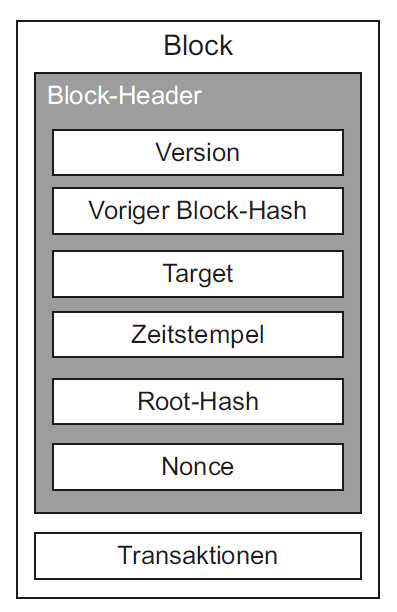
\includegraphics[width=0.35\linewidth]{images/blockchain_block.png}
    \caption{Aufbau eines Blocks \parencite[S. 11]{Fill_BlockchainGrundlagen}}
    \label{fig:block}
\end{figure}


\noindent Der Block-Header enthält Informationen, wie zum Beispiel den Hash des vorherigen Blocks, die Schwierigkeit, den Zeitstempel und die Nonce. Die Schwierigkeit wird durch das \textit{Target}-Feld angegeben und beschreibt, wie schwer es ist, das kryptografische Puzzle zu lösen und damit auch wie schwer es ist, einen neuen Block an die Blockchain anzuhängen. Die Suche nach der Lösung dieses Puzzles wird auch als \textit{Mining} bezeichnet. Der erste, der das Puzzle löst, präsentiert als Beweis dieser Lösung die sogenannte \textit{Nonce}. Die Nonce ist eine zufällige Zahl, die bei der Lösung des Puzzles verwendet wird und aufwändig zu berechnen ist. Nachdem diese neue Version der Blockchain (mit dem neu angehängten Block) an alle anderen Teilnehmer verteilt wurde, kann jeder Teilnehmer überprüfen, ob die Lösung korrekt ist. Durch den Verweis im Block-Header auf den vorherigen Block entsteht die oben erwähnte Kette von Blöcken - die Blockchain (siehe Abbildung \ref{fig:chain_of_blocks}) \parencite[S. 10-12]{Fill_BlockchainGrundlagen}.

\begin{figure}[H]
    \centering
    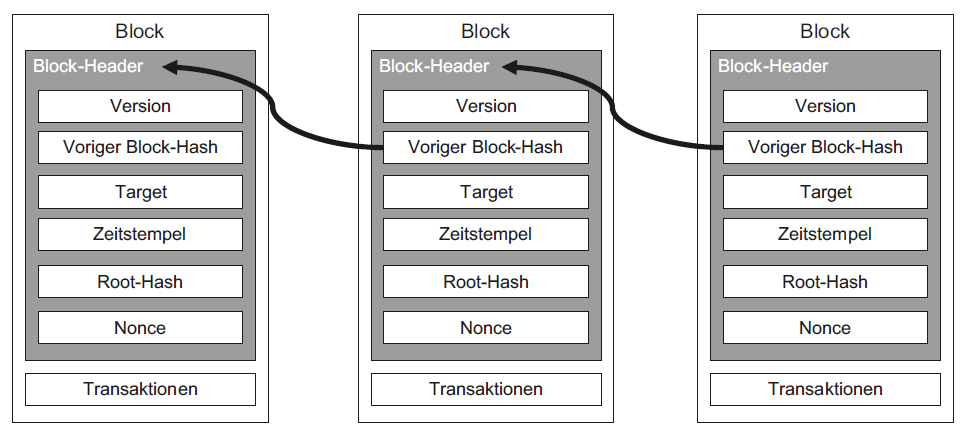
\includegraphics[width=0.9\linewidth]{images/chain_of_blocks.png}
    \caption{Kette aus Blöcken \parencite[S. 12]{Fill_BlockchainGrundlagen}}
    \label{fig:chain_of_blocks}
\end{figure}


\subsection{Kombination von technologischen Ansätzen}
\label{subsec:cryptography_basics}

Wie zu Beginn des Abschnitts \ref{sec:blockchain_basics} \textit{\nameref{sec:blockchain_basics}} bereits erwähnt, ist die Blockchain das Resultat der Kombination verschiedener Technologien. Diese Technologien werden in diesem Abschnitt erläutert.


\subsubsection{Kryptografie}

Aus der Kryptografie werden Hash-Funktionen, kryptografische Puzzles, Hash-Bäume und digitale Signaturen verwendet. 

Hash-Funktionen gewährleisten die Integrität der Blöcke. Wie dies durch Hash-Funktionen erreicht wird, wurde in Abschnitt \ref{subsec:integritaet_signatur} \textit{\nameref{subsec:integritaet_signatur}} erläutert. 

Kryptografische Puzzles werden dazu verwendet, um die Schwierigkeit beim Mining zu erhöhen. Dabei soll mittels Hash-Funktionen ein bestimmter Ausgabewert gefunden werden. Laut der Definition einer kryptografischen Hash-Funktion (siehe Abschnitt \ref{subsec:integritaet_signatur} \textit{\nameref{subsec:integritaet_signatur}}) ist es nicht möglich, von der Ausgabe auf die Eingabe zu schließen. Daher kann die gesuchte Eingabe nur durch Ausprobieren gefunden werden. Die Schwierigkeit kann durch die Anzahl der Nullen, die am Anfang des Hash-Wertes stehen müssen, angegeben werden. Je mehr Nullen am Anfang des Hash-Wertes stehen müssen, desto schwieriger ist es, die Lösung zu finden, da dadurch der Lösungsraum verkleinert wird \parencites[S. 6-7]{Fill_BlockchainGrundlagen}[S. 320]{Antonopoulos_MasteringEthereum}.

Ein \textit{Merkle-Baum} ist ein binärer Baum, bei dem jeder Knoten den Hash-Wert seiner Kinder enthält. Der nach seinem Erfinder Ralph Merkle benannte Hash-Baum wird in der Blockchain zum Aufbau von Datenstrukturen verwendet. Der Hash-Wert der Wurzel des Baumes wird auch als \textit{Root-Hash} oder \textit{Merkle-Root} bezeichnet (siehe Abbildung \ref{fig:block}: \textit{Root-Hash}). Wenn sich ein Blatt des Baumes ändert, ändert sich auch der Hash-Wert der Wurzel. Dadurch kann kontrolliert werden, ob sich an einer beliebigen Stelle Daten geändert haben. Wenn sich die Daten geändert haben, ändert sich auch der Root-Hash. Wenn sich die Daten nicht geändert haben, bleibt der Root-Hash gleich. Dadurch kann die Integrität der Daten überprüft werden \parencite[S. 7-8]{Fill_BlockchainGrundlagen}. In Abbildung \ref{fig:merkle_tree} ist der Aufbau eines Merkle-Baumes zu sehen, der aus vier Transaktionen besteht.

\begin{figure}[H]
    \centering
    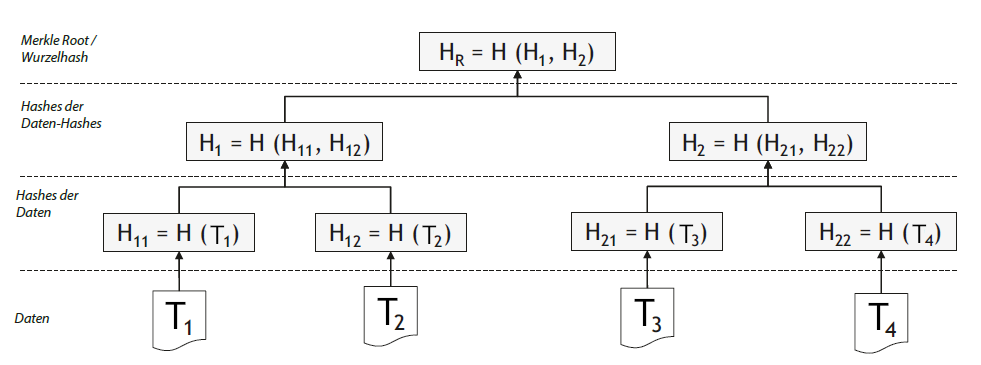
\includegraphics[width=0.9\linewidth]{images/merkle_tree_modified.png}
    \caption{Aufbau eines Merkle-Baumes (in Anlehnung an \cite[S. 8]{Fill_BlockchainGrundlagen})}
    \label{fig:merkle_tree}
\end{figure}

\noindent Von jeder Transaktion $T_{1}$, $T_{2}$, $T_{3}$ und $T_{4}$ wird ein Hash-Wert berechnet und in einem Blatt des Baumes gespeichert. Die Hash-Werte der Blätter werden dann paarweise gehasht und in den Knoten darüber gespeichert. Dieser Vorgang wird solange wiederholt, bis nur noch ein Knoten übrig ist. Dieser Knoten enthält den Root-Hash. Sollte sich eine Transaktion ändern, ändert sich auch der Root-Hash. Außerdem kann bewiesen werden, dass beispielsweise $T_{2}$ Teil des Baumes ist, indem mit dem Hash-Wert von $T_{2}$ und den Hash-Werten von $T_{1}$, $T_{3}$ und $T_{4}$ versucht wird, den Root-Hash zu berechnen. Wenn der berechnete Root-Hash mit dem tatsächlichen Root-Hash übereinstimmt, ist bewiesen, dass $T_{2}$ Teil des Baumes ist \parencite[S. 9]{Fill_BlockchainGrundlagen}.

Die folgende Abbildung zeigt das Zusammenspiel von Blöcken, Transaktionen und Merkle-Bäumen:

\begin{figure}[H]
    \centering
    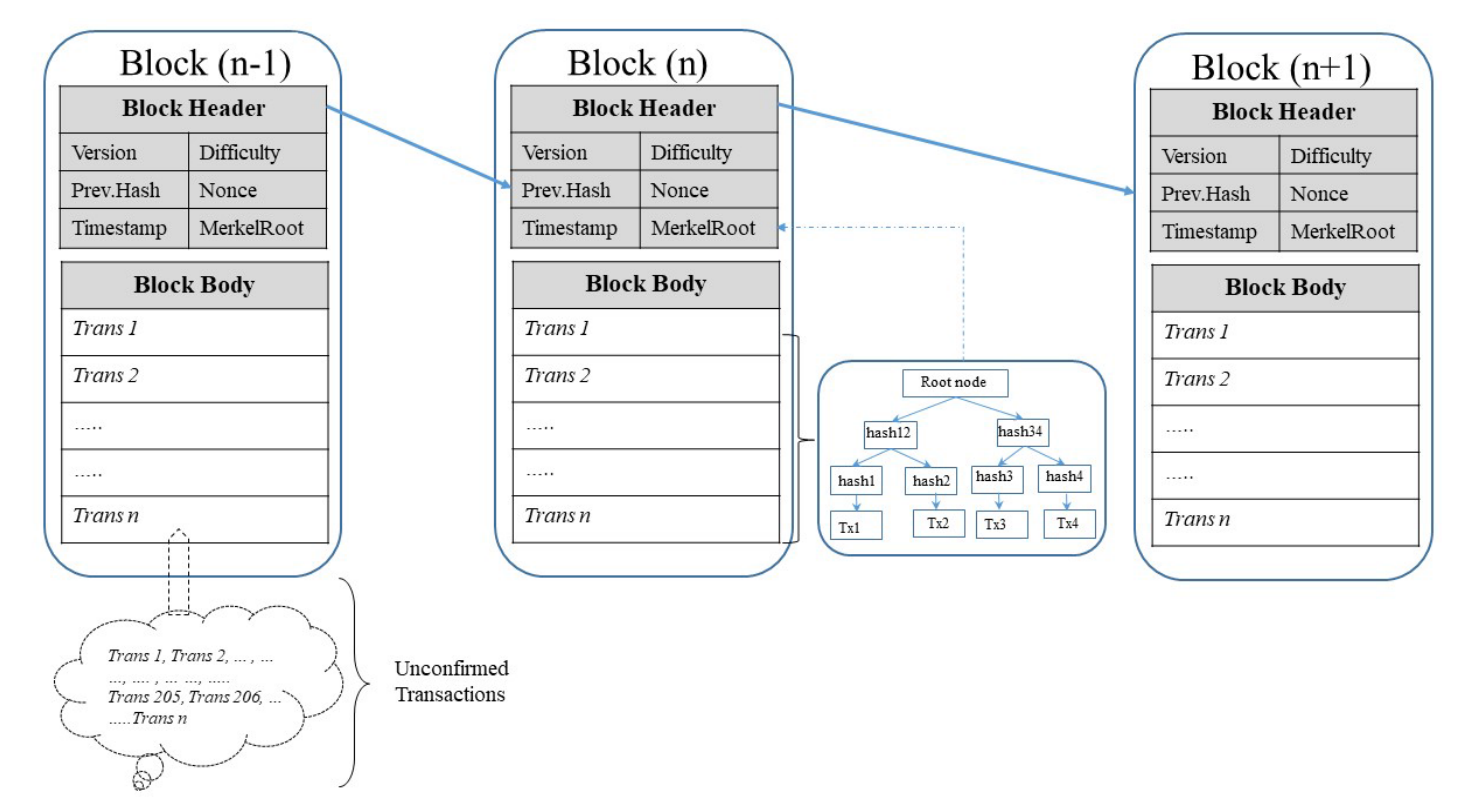
\includegraphics[width=1\linewidth]{images/chain_of_blocks_with_merkle_tree.png}
    \caption{Verkettete Blöcke mit Transaktionen im Block-Body \parencite[S. 95035]{Nam_51PercentAttacks}}
    \label{fig:chain_of_blocks_with_merkle_tree}
\end{figure}


\noindent Eine weitere Technologie aus der Kryptografie, die in der Blockchain verwendet wird, sind digitale Signaturen. Digitale Signaturen werden verwendet, um die Authentizität (siehe \ref{subsec:integritaet_signatur} \textit{\nameref{subsec:integritaet_signatur}}) von Daten zu gewährleisten \parencite[S. 9-10]{Fill_BlockchainGrundlagen}. Im Falle der Blockchain bedeutet das, dass die Transaktionen, die in einem Block enthalten sind, mit einer digitalen Signatur versehen werden. Dadurch wird den Benutzern der Blockchain garantiert, dass die Transaktionen von dem Besitzer des privaten Schlüssels signiert wurden. Wenn ein Angreifer versucht, die Transaktionen zu manipulieren, wird dies von den anderen Teilnehmern bemerkt, da die Transaktionen nicht mehr mit der digitalen Signatur übereinstimmen \parencite[S. 10]{Fill_BlockchainGrundlagen}.


\subsubsection{Dezentrale Netzwerke}

Blockchains machen sich eine weitere Technologie zunutze: dezentrale Netzwerke. Sie basieren auf einem Peer-to-Peer-Netzwerk, bei dem alle Teilnehmer gleichberechtigt sind (siehe \ref{subsec:peer_to_peer_technologie} \textit{\nameref{subsec:peer_to_peer_technologie}}). Es gibt keinen zentralen Server, der die Daten verwaltet. Stattdessen werden die Daten auf allen Teilnehmern des Netzwerkes gespeichert. Wenn ein Teilnehmer Daten an das Netzwerk senden möchte, sendet er die Daten an alle anderen Teilnehmer des Netzwerkes. Wenn ein Teilnehmer Daten vom Netzwerk empfangen möchte, empfängt er die Daten von allen anderen Teilnehmern des Netzwerkes. Dadurch ist es nicht möglich, das Netzwerk zu manipulieren, da die Daten auf allen Teilnehmern des Netzwerkes gespeichert sind. Wenn ein Teilnehmer versucht, die Daten zu manipulieren, wird dies von den anderen Teilnehmern bemerkt und die manipulierten Daten werden nicht akzeptiert \parencite[S. 10/31]{Fill_BlockchainGrundlagen}.


\subsubsection{Konsensmechanismen}
\label{consensus_mechanisms}

Durch die Dezentralität der Blockchain ist es möglich, dass die Teilnehmer des Netzwerkes unterschiedliche Daten haben. Es muss also eine Möglichkeit geben, sich auf einen, für alle \textit{richtigen}, gemeinsamen Zustand zu einigen. Dafür werden sogenannte \textit{Konsensmechanismen} verwendet. Dieser Zustand kann beispielsweise die Reihenfolge der getätigten Transaktionen sein. Wenn sich die Teilnehmer nicht auf einen gemeinsamen \textit{Konsens} einigen können, kann das Netzwerk nicht funktionieren. Die Aufgabe der Konsensmechanismen ist es also, einen gemeinsamen Zustand zu finden. Die beiden bekanntesten Konsensmechanismen sind \textit{Proof-of-Work} und \textit{Proof-of-Stake} \parencite[S. 87]{Alam_BlockchainConsensusMechanism}.

Der \textit{Proof-of-Work} (kurz: \textit{PoW}) ist der Konsensmechanismus, der in der Bitcoin-Blockchain verwendet wird. Bitcoin wurde 2008 von Satoshi Nakamoto, dessen wahre Identität bis heute unbekannt ist, in einem Whitepaper vorgestellt und ist die erste dezentrale Kryptowährung \parencites{Nakamoto_Bitcoin}{Zhang_DoubleSpendingWithASybilAttack}. Der PoW besteht aus dem bereits in Abschnitt \ref{subsec:blockchain_definition} \textit{\nameref{subsec:blockchain_definition}} beschriebenen kryptografischen Puzzle. Das Lösen des Puzzles durch einen beliebigen Teilnehmer dient als Nachweis für geleistete Rechenarbeit - daher die Bezeichnung \textit{Proof-of-Work} \parencite[S. 27]{Brünnler_BlockchainKurzGut}. Ein großer Nachteil bei Proof-of-Work ist der hohe Energieverbrauch, der dem hohen Rechenaufwand zum Lösen des Puzzles geschuldet ist \parencite{Zhang_EvaluationOfEnergyConsumptionInBlockChains}. Die Website \textit{Digiconomist.net} führt einen Energieindex für Bitcoin, der den Energieverbrauch von Bitcoin in Relation zu verschiedenen Ländern setzt. Aktuell benötigt Bitcoin jährlich rund $144$ TWh, was ungefähr dem jährlichen Energieverbrauch von Schweden entspricht \parencite{Digiconomist_BitcoinEnergyConsumption}.

Der \textit{Proof-of-Stake} (kurz: \textit{PoS}) ist ein alternativer Konsensmechanismus. Im Gegensatz zum PoW wird beim PoS kein kryptografisches Puzzle gelöst, um einen neuen Block anzuhängen. Stattdessen müssen Teilnehmer, die einen neuen Block anhängen möchten, einen Einsatz (engl. \textit{Stake}) in Form von Kryptowährung hinterlegen. Die Wahrscheinlichkeit dafür ist proportional zum hinterlegten Einsatz. Wenn ein Teilnehmer (auch \textit{Validator} genannt) ausgewählt wurde und er einen weiteren Block anhängt, wird dieser von den anderen Validatoren des Netzwerkes überprüft. Wenn der angehängte Block gültig ist, bedeutet das, dass er keine ungültigen Transaktionen enthält und der Teilnehmer seinen Stake wieder erstattet bekommt. Wenn der Block allerdings von den anderen Validatoren als ungültig erkannt wird, verliert der Teilnehmer seinen Stake. Dadurch wird sichergestellt, dass die Teilnehmer des Netzwerkes ehrlich sind und keine ungültigen Blöcke anhängen \parencites[S. 96-97]{Kapengut_EthereumTransitionToProofOfStake}[S. 34]{Meinel_BlockchainHypeInnovation}[S. 320-321]{Antonopoulos_MasteringEthereum}.

Die beiden Konsensmechanismen unterscheiden sich grundlegend in ihrer Funktionsweise. PoW, das von Bitcoin genutzt wird, erfordert von Minern, komplexe mathematische Rätsel zu lösen, welche rechenintensiv sind und deshalb viel Energie benötigen. Der Miner, der das Rätsel zuerst löst, kann einen neuen Block hinzufügen und erhält eine Belohnung in Form von Kryptowährung \parencite{Fill_BlockchainGrundlagen}. PoW ist bekannt für:

\begin{itemize}
    \item Energieintensität: PoW erfordert hohe Rechenleistung und verbraucht viel Energie, was Umweltbedenken aufwirft \parencite[S. 96-97]{Kapengut_EthereumTransitionToProofOfStake}.
    \item Sicherheit: Das Netzwerk ist widerstandsfähig gegen Angriffe, da ein Angreifer die Kontrolle über die Mehrheit der Rechenleistung benötigt, um das Netzwerk zu übernehmen, was sehr teuer ist.
\end{itemize}

\noindent Im Gegensatz dazu nutzt PoS den Besitz von Kryptowährung als Sicherheitsfaktor. Validatoren werden auf Basis ihres Einsatzes (Stake) ausgewählt, um Transaktionen zu bestätigen \parencites[S. 34]{Meinel_BlockchainHypeInnovation}[S. 320-321]{Antonopoulos_MasteringEthereum}. PoS bietet:

\begin{itemize}
    \item Energieeffizienz: PoS ist energieeffizienter, da es nicht die immense Rechenleistung von PoW erfordert \parencite[S. 96-97]{Kapengut_EthereumTransitionToProofOfStake}.
    \item Sicherheit durch Einsätze: Die Validatoren haben einen Anreiz, sich ehrlich zu verhalten, da sie ihren Einsatz verlieren könnten, wenn sie betrügen \parencites[S. 34]{Meinel_BlockchainHypeInnovation}[S. 320-321]{Antonopoulos_MasteringEthereum}.
\end{itemize}

\noindent Zusammenfassend: PoW ist energieintensiver und bietet Sicherheit durch Rechenleistung, während PoS energieeffizienter ist und Sicherheit durch den Einsatz von Kryptowährung gewährleistet. Beide Mechanismen haben Vor- und Nachteile, und ihre Anwendung hängt von den spezifischen Anforderungen und Zielen des jeweiligen Blockchain-Netzwerks ab.


\subsection{Sicherheit von Blockchain-Technologie}

Die Blockchain gilt als sicher, da sie auf verschiedenen kryptografischen Technologien basiert (siehe Abschnitt \ref{subsec:cryptography_basics} \textit{\nameref{subsec:cryptography_basics}}). Hinzu kommt die Unveränderlichkeit der Blockchain, was bedeutet, dass einmal geschriebene Transaktionen nach der Bestätigung durch den Konsensmechanismus als unveränderlich gelten und die Blockchain damit eine Fälschungssicherheit bietet \Parencites[S. 1-2]{Landerreche_ImmutabilityOfBlockchains}[S. 70]{Brünnler_BlockchainKurzGut}. Da Blöcke durch kryptografische Hashes verknüpft sind, wäre eine nachträgliche Änderung äußerst rechenintensiv und offensichtlich, da alle nachfolgenden Blöcke ebenfalls verändert werden müssten \Parencite[S. 12]{Fill_BlockchainGrundlagen}. Zusätzlich zu diesen Grundlagen sind Sicherheitsmaßnahmen entscheidend. Anreizstrukturen belohnen Miner/Validatoren für ehrliches Handeln und bestrafen bösartiges Verhalten, was als Abschreckung dient \parencite[S. 320-321]{Antonopoulos_MasteringEthereum}. Die dezentrale Natur der Blockchain macht sie widerstandsfähig gegen verschiedene Angriffe, da es keinen einzelnen Angriffspunkt, wie beispielsweise einen Server, gibt \parencite[S. 31]{Fill_BlockchainGrundlagen}.

Letztendlich unterliegt die Sicherheit der Blockchain jedoch keinem absoluten Schutz. Risiken wie 51\%-Angriffe oder Schwachstellen in spezifischen Implementierungen können weiterhin Bedrohungen darstellen. Daher sind kontinuierliche Forschung, Protokollaktualisierungen und bewährte Sicherheitspraktiken entscheidend, um Risiken zu minimieren und die Sicherheit der Blockchain weiter zu verbessern \parencites{Nam_51PercentAttacks}{Perez_SmartContractVulnerabilities}.


\subsection{Angriffe auf Blockchain}

Die Blockchain-Technologie ist nicht immun gegen Angriffe. Es gibt verschiedene Angriffe, die auf Blockchains durchgeführt werden können. Durch die Dezentralität kommen teilweise die gleichen Angriffe wie bei Peer-to-Peer-Netzwerken zum Einsatz. Die bekanntesten Angriffe sind der 51\%-Angriff, der Sybil-Angriff und für Ethereum 2.0 die Smart Contract Exploits \Parencites[S. 95034]{Nam_51PercentAttacks}[S. 251]{Douceur_SybilAttack}. Diese Angriffe werden in den folgenden Abschnitten erläutert.

\subsubsection{51\%-Angriff}

Ein 51\%-Angriff ist ein potenziell bedrohlicher Angriff auf eine Blockchain, bei dem eine einzelne Entität oder eine koordinierte Gruppe die Kontrolle über die Mehrheit der Rechenleistung (bei PoW) oder der Stake (bei PoS) eines Netzwerks erlangt. Dies könnte dazu führen, dass die Angreifer die Blockchain manipulieren, doppelte Ausgaben tätigen (auch als \textit{Double Spending} bekannt) oder Transaktionen zensieren können \Parencites[S. 95034]{Nam_51PercentAttacks}[S. 2]{Rosenfeld_DoubleSpending}. Dies gestaltet sich als sehr teuer, da die Angreifer die Kontrolle über die Mehrheit der Rechenleistung oder des Stakes erlangen müssen, was sehr viel Energie, Rechenleistung und Geld erfordert. Außerdem ist es sehr unwahrscheinlich, dass ein Angreifer die Kontrolle über die Mehrheit der Rechenleistung oder des Stakes erlangt, da die Blockchain sehr groß ist und es sehr viele Teilnehmer gibt.

\subsubsection{Smart Contract Exploits}

Smart Contracts sind Programme, die auf der Blockchain ausgeführt werden (siehe \ref{subsection:smart_contracts} \textit{\nameref{subsection:smart_contracts}}). Sie werden mit Hilfe einer Programmiersprache geschrieben, und wie auch bei jedem anderen Programm können auch Smart Contracts Fehler enthalten. Wenn ein Fehler in einem Smart Contract identifiziert wird, kann dieser Fehler ausgenutzt werden \Parencite[S. 1-2]{Perez_SmartContractVulnerabilities}. Ein Beispiel für einen Smart Contract Exploit ist der \textit{DAO Hack}, der im Juni 2016 stattfand. Der DAO Hack ist ein Angriff auf den Smart Contract \textit{The DAO}, der auf der Ethereum-Blockchain ausgeführt wurde. \textit{DAO} steht für \textit{Decentralized Autonomous Organization} (zu Deutsch: \textit{dezentralisierte autonome Organisation}). Dieser Smart Contract war ein dezentraler Risikokapitalfonds, der es den Teilnehmern ermöglichte, über die Verwendung der Gelder abzustimmen. Die Teilnehmer konnten Ether in den Smart Contract einzahlen und erhielten dafür \textit{DAO-Token}. Diese DAO-Token konnten verwendet werden, um über die Verwendung der Gelder abzustimmen. Wenn ein Teilnehmer seine DAO-Token zurückziehen wollte, konnte er dies tun, indem er den Smart Contract aufrief und seine DAO-Token gegen Ether eintauschte \parencite{Pratap_DAOHack}. 

Experten fanden jedoch eine Schwachstelle im Smart Contract, die es einem Angreifer ermöglichte, mehrmals DAO-Token gegen Ether einzutauschen. Der Angreifer nutzte diese Schwachstelle aus und tauschte seine DAO-Token mehrmals gegen Ether ein. Dadurch erhielt er mehr Ether, als er ursprünglich eingezahlt hatte. Der Angreifer konnte Ether im Wert von 50 Millionen US-Dollar stehlen. Um den Schaden zu begrenzen, wurde ein sogenannter \textit{Hard Fork} durchgeführt. Dabei wurde die Blockchain in zwei Versionen aufgeteilt. In der einen Version wurde der DAO Hack rückgängig gemacht und in der anderen Version nicht. Die Version, in der der DAO Hack rückgängig gemacht wurde, wurde von der Mehrheit der Teilnehmer verwendet und ist heute als Ethereum bekannt. Die Version, in der der DAO Hack nicht rückgängig gemacht wurde, wird heute als Ethereum Classic bezeichnet. Der DAO Hack ist ein lehrreiches Beispiel dafür, wie ein Fehler in einem Smart Contract ausgenutzt (engl. \textit{exploited}) werden kann, um große Summen an Geld zu stehlen \parencite{Price_DAOHack}.


\subsubsection{Sybil-Angriff}

Wie in Abschnitt \ref{subsubsec:sybil_or_eclipse_attack_p2p} \textit{\nameref{subsubsec:sybil_or_eclipse_attack_p2p}} bereits ausgeführt, ist ein Sybil-Angriff ein Angriff auf ein Peer-to-Peer-Netzwerk, bei dem ein einzelner Angreifer mehrere Identitäten verwendet, um das Netzwerk zu manipulieren. Da Blockchains auf Peer-to-Peer-Netzwerken basieren, sind sie ebenfalls anfällig für diese Art von Angriffen.  

\subsection{Ethereum}
\label{sec:ethereum_basics}

Ethereum ist eine der führenden Blockchain-Plattformen und wurde 2015 von Vitalik Buterin, Gavin Wood und anderen entwickelt. Im Gegensatz zu Bitcoin, das hauptsächlich als digitale Währung fungiert, ermöglicht Ethereum die Ausführung von Smart Contracts und die Entwicklung von dezentralen Anwendungen (engl. \textit{decentralized Applications}, kurz \textit{DApps}) \Parencites[S. 720]{Sorge_BitcoinZahlungsmittelDerZukunft}[S. 1-2]{Perez_SmartContractVulnerabilities}. Bis 2022 wurde als Konsensmechanismus Proof-of-Work verwendet, der jedoch 2022 durch Proof-of-Stake ersetzt wurde. Seitdem existieren zwei Versionen von Ethereum: \textit{Ethereum Classic} und \textit{Ethereum 2.0}. Ethereum Classic verwendet Proof-of-Work, während Ethereum 2.0 Proof-of-Stake verwendet \Parencite{EthereumClassic_ResearcherFAQs}.

Ether (ETH) ist die native Kryptowährung von Ethereum und wird für Transaktionen innerhalb des Netzwerks verwendet. Es dient auch als Anreiz für diejenigen, die an der Sicherung des Netzwerks durch Mining (bei PoW) oder Validierung (bei PoS) von Transaktionen beteiligt sind \parencite[S. 320-321]{Antonopoulos_MasteringEthereum}. Die Flexibilität von Ethereum und seine Fähigkeit, innovative Lösungen zu unterstützen, haben es zu einer der wichtigsten Plattformen in der Blockchain-Welt gemacht.

\subsection{Smart Contracts}
\label{subsection:smart_contracts}
% Smart Contracts werden per RPC aufgerufen.


Ein Smart Contract (zu Deutsch: \textit{intelligenter Vertrag}) ist im Grunde genommen ein selbstausführender Vertrag, der automatisch Aktionen auslöst, wenn bestimmte Bedingungen erfüllt sind \Parencite[S. 1-2]{Perez_SmartContractVulnerabilities}. Die Bezeichnung \textit{Smart Contract} ist eigentlich eine Fehlbezeichnung, da es sich weder um einen Vertrag im rechtlichen Sinne, noch um einen \textit{intelligenten} Vertrag handelt, doch der Begriff hat sich in der Blockchain-Community etabliert und wird deshalb weiterhin verwendet. Ein Lesezugriff auf einen Smart Contract ist kostenlos, ein Schreibzugriff hingegen kostet Geld, da die Transaktion in der Blockchain gespeichert werden muss. Dieses Geld wird als \textit{Gas} bezeichnet und ist eine Art Gebühr, die gezahlt werden muss, um die Rechenleistung des Netzwerks zu nutzen \Parencite[S. 127]{Antonopoulos_MasteringEthereum}. Um Gas zu erhalten, muss der Nutzer Ether eintauschen, die Währung der Ethereum-Blockchain.
Für das Protokoll dieser Arbeit wurden sowohl Lese- als auch Schreibzugriffe auf Smart Contracts implementiert (siehe Kapitel \ref{chap:entwurf_und_architektur} \textit{\nameref{chap:entwurf_und_architektur}}).

Die Plattform verwendet die objektorientierte Programmiersprache \textit{Solidity}, die speziell für Smart Contracts entwickelt wurde und stark an JavaScript angelehnt ist. Entwickler können mithilfe von Solidity Smart Contracts erstellen, die dann in der Ethereum-Blockchain ausgeführt werden und von jedem Teilnehmer des Netzwerks aufgerufen werden können \Parencite[S. 127-133]{Antonopoulos_MasteringEthereum}.
